\documentclass[a4paper,dvipdfmx,11pt,reqno]{amsart}
\usepackage{amsmath,amsthm,amssymb,mathrsfs,stmaryrd}
\usepackage{bm}
\usepackage{url}
\usepackage{color}
\usepackage{eucal}
\usepackage{slashed}
\usepackage{physics}
\usepackage{graphicx}
\usepackage{tikz}
\usepackage{tikz-cd}
\usetikzlibrary{intersections, calc, arrows, arrows.meta, shadows}
\usepackage[utf8]{inputenc} % for special characters
\usepackage[T1]{fontenc}
\usepackage[backend=biber,style=alphabetic,hyperref=true]{biblatex} % for bib latex
\addbibresource{six_functor_formalisms.bib}
\usepackage{geometry} % margin settings
\geometry{margin=1.0in}
\usepackage{enumitem} % item style
\setlist[enumerate]{itemsep=2pt,parsep=2pt,before={\parskip=2pt}}
\setlist[description]{style=standard}
\usepackage[colorlinks=true,hyperindex, linkcolor=magenta, pagebackref=false, citecolor=cyan,pdfpagelabels]{hyperref} % link colors
\usepackage{cleveref}

\renewcommand{\baselinestretch}{1.1} % change the space between lines

% hiragana yo and oy
\DeclareFontFamily{U}{dmjhira}{}
\DeclareFontShape{U}{dmjhira}{m}{n}{
  <-> dmjhira
}{}
\DeclareFontSubstitution{U}{dmjhira}{m}{n}
\newcommand{\yo}{\text{{\usefont{U}{dmjhira}{m}{n}\symbol{"48}}}}
\newcommand{\oy}{\text{{\reflectbox{\yo}}}}

% math definitions
\DeclareMathOperator{\Ob}{Ob}
\DeclareMathOperator{\Hom}{Hom}
\DeclareMathOperator{\Map}{Map}
\DeclareMathOperator{\myop}{op}
\DeclareMathOperator{\id}{id}
\DeclareMathOperator{\Id}{Id}
\DeclareMathOperator{\h}{h}
\DeclareMathOperator{\N}{N}
\DeclareMathOperator*{\colim}{colim}
\DeclareMathOperator{\Fun}{Fun}
\DeclareMathOperator{\FunL}{Fun^{L}}
\DeclareMathOperator{\Ind}{Ind}
\DeclareMathOperator{\supp}{supp}
\DeclareMathOperator{\Supp}{Supp}
\DeclareMathOperator{\Mul}{Mul}
\DeclareMathOperator{\Ker}{Ker}
\renewcommand{\ev}{\mathrm{ev}}
\newcommand{\bbN}{\mathbb{N}}
\newcommand{\bbR}{\mathbb{R}}
\newcommand{\bbZ}{\mathbb{Z}}
\newcommand{\otimesL}{\mathop{\otimes}\limits^{\mathrm{L}}}
\renewcommand{\Im}{\mathrm{Im}}

% categories (using mathcal)
\newcommand{\A}{\mathcal{A}}
\newcommand{\B}{\mathcal{B}}
\newcommand{\C}{\mathcal{C}}
\newcommand{\D}{\mathcal{D}}
\newcommand{\E}{\mathcal{E}}
\newcommand{\F}{\mathcal{F}}
\newcommand{\G}{\mathcal{G}}
\newcommand{\I}{\mathcal{I}}
\newcommand{\J}{\mathcal{J}}
\newcommand{\V}{\mathcal{V}}
\newcommand{\W}{\mathcal{W}}
\renewcommand{\H}{\mathcal{H}}
\renewcommand{\O}{\mathcal{O}}
\renewcommand{\P}{\mathcal{P}}
\renewcommand{\S}{\mathcal{S}}

% categories (using math rm)
\newcommand{\Ab}{\mathrm{Ab}}
\newcommand{\An}{\mathrm{An}}
\newcommand{\AN}{\mathrm{AN}}
\newcommand{\Cat}{\mathrm{Cat}}
\newcommand{\CMon}{\mathrm{CMon}}
\newcommand{\CAT}{\mathrm{CAT}}
\newcommand{\Open}{\mathrm{Open}}
\newcommand{\PrL}{\mathrm{Pr}^{\mathrm{L}}}
\newcommand{\Pshv}{\mathrm{Pshv}}
\newcommand{\Shv}{\mathrm{Shv}}
\newcommand{\TwAr}{\mathrm{TwAr}}
\newcommand{\Corr}{\mathrm{Corr}}
\newcommand{\Fin}{\mathrm{Fin}}
\newcommand{\core}{\mathrm{core}}

\renewcommand{\angle}[1]{\left\langle #1 \right\rangle}

% theorem style (using definition style)
\newtheorem{theorem}{Theorem}[section]
\theoremstyle{definition}
\newtheorem{definition}[theorem]{Definition}
\newtheorem{conjecture}[theorem]{Conjecture}
\newtheorem{construction}[theorem]{Construction}
\newtheorem{corollary}[theorem]{Corollary}
\newtheorem{example}[theorem]{Example}
\newtheorem{lemma}[theorem]{Lemma}
\newtheorem{notation}[theorem]{Notation}
\newtheorem{proposition}[theorem]{Proposition}
\newtheorem{remark}[theorem]{Remark}

% Customizing clever-ref 
\crefname{notation}{Notation}{Notations}

% ------------------------------------------------------

\begin{document}

\title{A Note on Six-Functor Formalisms}
\author{Keima Akasaka}
\maketitle 

\begin{abstract}
  We summarize key concepts and results on six-functor formalisms, focusing on their foundational aspects.
\end{abstract} 

\setcounter{tocdepth}{2} % show depth in contents
\tableofcontents   

\section{Introduction}

The aim of this note is to explain \textit{what a six-functor formalism is}. 
The concept of six functors for sheaves originated in Grothendieck's work, and these are often referred to as Grothendieck's six operations.

The first such formalism was developed to establish the \'{e}tale cohomology of schemes, as formulated by Yifeng Liu and Weizhe Zheng \cite{LZ17}.
A subsequent formalism, intended for coherent cohomology of schemes, was provided by Dennis Gaitsgory and Nick Rozenblyum \cite{GR17}. 
The former approach is based on heavy combinatorics of specific simplicial sets, while the latter uses the framework of $(\infty,2)$-categories. 
More recently, Lucas Mann \cite{Mann22} has proposed a refined definition that combines favorable aspects of both methods.
We will present Mann's definition after reviewing classical sheaf theory and Grothendieck's six operations.

In \cref{sec.classical_sheaf_theory}, we review classical sheaf theory with a focus on the proper base change theorem and projection formula. 
(The abstract theory of derived categories and derived functors is summarized in \cref{sec.derived_categories}.) 
In \cref{sec.six_functors_formalisms}, we introduce the six-functor formalism and present some fundamental propositions.

\subsection{Notation}

We let 
\begin{itemize}
  \item $\Ab$ denote the category of abelian groups.
  \item $\Pshv(X)$ denote the category of presheaves on a topological space $X$.
  \item $\Shv(X)$ denote the category of sheaves on a topological space $X$.
  \item $\Cat$ denote the $\infty$-category of small $\infty$-categories.
  \item $\CMon(\C)$ denote the category of commutative monoids on a category $\C$.
\end{itemize}


\section{Classical Sheaf Theory} \label{sec.classical_sheaf_theory}

In this section, we review the fundamental concepts and results of classical sheaf theory and Grothendieck's six functors. 
In \cref{subsec.the_category_of_sheaves}, we cover basic notions of the category of sheaves and the global section functor. 
In \cref{subsec.six_operations_on_the_category,subsec.six_operations_on_the_derived_category}, we construct the six functors on the (derived) category of sheaves. 
In \cref{subsec.remarkable_results}, we highlight key results in sheaf theory: the proper base change theorem and projection formula. 
% Finally, in \cref{subsec.poincare_duality}, we discuss classical Poincar\'{e} duality.

\subsection{The Category of Sheaves} \label{subsec.the_category_of_sheaves}

\begin{definition}
  Let $X$ be a topological space.
  An (\textit{abelian}) \textit{presheaf} on $X$ is a functor 
  \begin{align*}
    F : \Open(X)^{\myop} \to \Ab.
  \end{align*}
  A \textit{morphism of presheaves} is a natural transformation between presheaves.
  We let $\Pshv(X)$ denote the category of presheaves on $X$ with morphisms of presheaves, and refer to it as the \textit{category of presheaves} on $X$.
\end{definition}

\begin{definition}
  Let $X$ be a topological space, and let $F$ be a presheaf on $X$.
  We will say that $F$ is a \textit{sheaf} if, for every complete full subcategory $\mathcal{U}$ of $\Open(X)$, $F$ carries every colimit which exists in $\mathcal{U}$ to a limit in $\Ab$.
  We let $\Shv(X)$ denote the full subcategory of $\Pshv(X)$ spanned by sheaves on $X$, and refer to it as the \textit{category of sheaves} on $X$.
\end{definition}

\begin{proposition}
  Let $X$ be a topological space.
  By the adjoint functor theorem, the inclusion $\Shv(X) \subseteq \Pshv(X)$ admits a left adjoint, called the \textit{sheafification functor}
  \begin{align*}
    (-)^{+} : \Pshv(X) \to \Shv(X).
  \end{align*}
\end{proposition}

\begin{definition}
  Let $X$ be a topological space, and let $F$ be a sheaf on $X$.
  For an open subset $U$ of $X$, an element of $F(U)$ is called a \textit{section} on $U$ of $F$.
  In particular, an element of $F(X)$ is called a \textit{global section} of $F$.
  The construction $F \mapsto F(X)$ defines the \textit{global section functor}
  \begin{align*}
    \Gamma(X;-) : \Shv(X) \to \Ab.
  \end{align*}
\end{definition}

\begin{definition}
  Let $X$ be a topological space, $F$ be a sheaf on $X$, $U$ be an open subset of $X$, and let $s$ be a section on $U$ of $F$.
  A \textit{support} $\supp(s)$ of $s$ is the complement set $U \backslash V$, where $V$ is the largest open subset of $X$ on which $s|_{V}=0$.
\end{definition}

We can define the \textit{kernel sheaf} $\Ker \varphi$ and the \textit{image sheaf} $\Im \varphi$ for a morphism $\varphi$ of sheaves, and they endow an abelian category structure on the category of sheaves.
Then we can consider exact sequences of sheaves.

\begin{proposition}
  Let $X$ be a topological space.
  Then the category $\Shv(X)$ is an abelian category which has enough injectives.
\end{proposition}

\begin{definition}
  A sequence of sheaves $F \xrightarrow{\varphi} G \xrightarrow{\psi} H$ is called \textit{exact} if it satisfies $\Im \varphi = \Ker \psi$.
\end{definition}

\begin{proposition}
  Let $X$ be a topological space.
  Then the global section functor $\Gamma(X;-) : \Shv(X) \to \Ab$ is left exact.
  That is, for every short exact sequence of sheaves $0 \to F \to G \to H \to 0$, $0 \to \Gamma(X;F) \to \Gamma(X;G) \to \Gamma(X;H)$ is exact in $\Ab$.
\end{proposition}

\subsection{Grothendieck's Six Functors on the Category of Sheaves} \label{subsec.six_operations_on_the_category}

In this section, we recall Grothendieck's six functors.
We first discuss how to construct a new sheaf from the given sheaves.

\begin{definition}
  Let $X$ be a topological space, and let $F$ and $G$ be sheaves on $X$.
  For every open subset $U$ of $X$, we define 
  \begin{align*}
    \underline{\Hom}(F,G)(U) := \Hom_{\Shv(X)}(F|_{U},G|_{U}),
  \end{align*}
  which induces a sheaf $\underline{\Hom}(F,G)$ on $X$.
  The construction $(F,G) \mapsto \underline{\Hom}(F,G)$ defines a bifunctor 
  \begin{align*}
    \underline{\Hom} : \Shv(X)^{\myop} \times \Shv(X) \to \Shv(X).
  \end{align*} 
  We will refer to it as the \textit{sheaf hom functor}.
\end{definition}

\begin{definition}
  Let $X$ be a topological space, and let $F$ and $G$ be sheaves on $X$.
  For every open subset $U$ of $X$, we define 
  \begin{align*}
    F \otimes' G(U) := F(U) \otimes_{\bbZ} G(U),
  \end{align*}
  which induces a presheaf $F \otimes' G$ on $X$.
  We let $F \otimes G := (F \otimes' G)^{+}$ denote the sheafification of $F \otimes' G$.
  The construction $(F,G) \mapsto F \otimes G$ defines a bifunctor 
  \begin{align*}
    \otimes : \Shv(X) \times \Shv(X) \to \Shv(X).
  \end{align*}
  We will refer to it as the \textit{tensor product functor}.
\end{definition}

\begin{proposition}
  Let $X$ be a topological space.
  Then there exists the following adjunction: 
  For every objects $F,G$ and $H$ of $\Shv(X)$, we have an isomorphism
  \begin{align*}
    \Hom_{\Shv(X)}(F \otimes G,H) \simeq \Hom_{\Shv(X)}(F,\underline{\Hom}(G,H)).
  \end{align*}
\end{proposition}

\begin{proposition}
  The tensor product functor $\otimes$ is right exact, and the sheaf hom functor $\underline{\Hom}$ is left exact. 
\end{proposition}

We next study the operators which transform sheaves along a continuous map between topological spaces.

\begin{definition}
  Let $f : X \to Y$ be a continuous map of topological spaces, and let $F$ be a sheaf on $X$.
  For every open subset $V$ of $Y$, we define 
  \begin{align*}
    f_{\ast}F(V) := \Gamma(f^{-1}(V);F) =  F(f^{-1}(V)),
  \end{align*}
  which induces a sheaf $f_{\ast}F$ on $Y$.
  The construction $F \mapsto f_{\ast}F$ defines a functor 
  \begin{align*}
    f_{\ast} : \Shv(X) \to \Shv(Y).
  \end{align*}
  We will refer to it as the \textit{direct image functor} or the \textit{pushout functor}.
  \[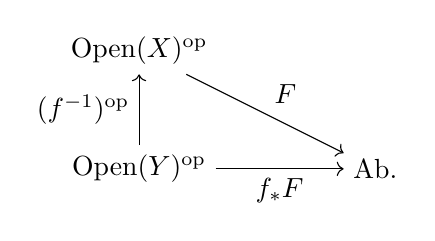
\begin{tikzpicture}[auto,->] 
    \node (tl) at (0,1.5) {$\Open(X)^{\myop}$}; 
    \node (bl) at (0,0) {$\Open(Y)^{\myop}$}; 
    \node (br) at (3,0) {$\Ab.$}; 
    % horizontal line 
    \draw (bl) -- node[swap] {$f_{\ast}F$} (br); 
    % vertical line
    \draw (bl) -- node {$(f^{-1})^{\myop}$} (tl);
    % from tl to br
    \draw (tl) -- node {$F$} (br); 
  \end{tikzpicture}\]
\end{definition}

We can construct a left adjoint functor to the direct image functor using the left Kan extension.

\begin{definition}
  Let $f : X \to Y$ be a continuous map of topological spaces, and let $G$ be a sheaf on $Y$.
  For every open subset $U$ of $X$, we define 
  \begin{align*}
    f'G(U) := \colim\limits_{f(U) \subset V} G(V),
  \end{align*}
  which induces a presheaf $f'G$ on $X$.
  We let $f^{\ast}G := (f'G)^{+}$ denote the sheafification of $f'G$.
  The construction $G \mapsto f^{\ast}G$ defines a functor 
  \begin{align*}
    f^{\ast} : \Shv(Y) \to \Shv(X).
  \end{align*}
  We will refer to it as the \textit{inverse image functor} or the \textit{pullback functor}.
  \[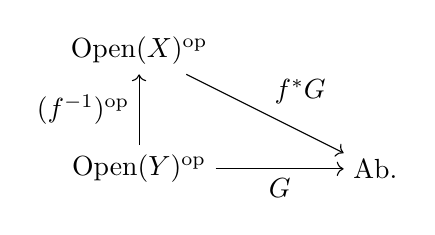
\begin{tikzpicture}[auto,->] 
    \node (tl) at (0,1.5) {$\Open(X)^{\myop}$}; 
    \node (bl) at (0,0) {$\Open(Y)^{\myop}$}; 
    \node (br) at (3,0) {$\Ab.$}; 
    % horizontal line 
    \draw (bl) -- node[swap] {$G$} (br); 
    % vertical line
    \draw (bl) -- node {$(f^{-1})^{\myop}$} (tl);
    % from tl to br
    \draw (tl) -- node {$f^{\ast}G$} (br); 
  \end{tikzpicture}\]
\end{definition}

\begin{proposition}
  Let $f : X \to Y$ be a continuous map of topological spaces.
  Then there exists the following adjunction 
  \begin{align*}
    f^{\ast} : \Shv(Y) \rightleftarrows \Shv(X) : f_{\ast}.
  \end{align*}
\end{proposition}

\begin{proposition}
  Let $f : X \to Y$ be a continuous map of topological spaces.
  Then the inverse image functor $f^{\ast}$ is exact, and the direct image functor $f_{\ast}$ is left exact.
\end{proposition}

In the rest of this section, we will consider the fifth functor, the \textit{proper direct image functor}.
It does not admit a right adjoint functor in the setting of the category of sheaves. 
From here all topological spaces are assumed to be (finite-dimensional) locally compact Hausdorff.

\begin{definition}
  Let $f : X \to Y$ be a continuous map of topological spaces.
  We will say that $f$ is \textit{proper} if, for every compact subset $K$ of $Y$, the inverse image $f^{-1}(K)$ is a compact subset of $X$.  
\end{definition}

The properness of continuous maps can be verified locally; 
in other words, properness is a local property.

\begin{definition}
  Let $f : X \to Y$ be a continuous map of topological spaces, and let $F$ be a sheaf on $X$.
  For every open subset $V$ of $Y$, we define 
  \begin{align*}
    f_{!}F(V) := \{s \in f_{\ast}F(V) ~|~ f|_{\supp(s)} : \supp(s) \to V \text{ is proper}\},
  \end{align*}
  which induces a sheaf $f_{!}F$ on $Y$.
  The construction $F \mapsto f_{!}F$ defines a functor 
  \begin{align*}
    f_{!} : \Shv(X) \to \Shv(Y).
  \end{align*}
  We will refer to it as the \textit{proper direct image functor}.
\end{definition}

\begin{remark}
  Let $f : X \to Y$ be a continuous map of topological spaces.
  Is there a right adjoint functor $f^{!} : \Shv(Y) \to \Shv(X)$ to the proper direct image functor $f_{!}$?
  The answer is "No," except in the case where $f$ is an inclusion of closed subsets. 
  This is because $f_{!}$ is not exact.
  However, this problem will be solved in the setting of the derived category of sheaves.
\end{remark}

\subsection{Grothendieck's Six Functors on the Derived Category of Sheaves} \label{subsec.six_operations_on_the_derived_category}

In this section, we consider Grothendieck's six functors in the setting of derived categories (see \cref{sec.derived_categories} for notations).
We first consider the derived functors of the sheaf hom functor $\underline{\Hom}$ and the tensor product functor $\otimes$. 

\begin{definition}
  Let $X$ be a topological space, and let $F$ and $G$ be objects of $C(\Shv(X))$.
  For every $n \geq 0$, we define 
  \begin{align*}
    \underline{\Hom}^n(F,G):= \prod_{i \in \bbZ} \underline{\Hom}(F^i,G^{n+i}),
  \end{align*}
  which induces a bifunctor $\underline{\Hom}^{\bullet} : K(\Shv(X))^{\myop} \times K(\Shv(X)) \to K(\Shv(X))$.
  Moreover, it induces the right derived functor 
  \begin{align*}
    \bbR \underline{\Hom} : D(X)^{\myop} \times D(X) \to D(X)
  \end{align*}
  of the sheaf hom functor $\underline{\Hom} : \Shv(X)^{\myop} \times \Shv(X) \to \Shv(X)$.
  It can be calculated as follows:
  For every objects $F$ and $G$ of $D(X)$, $\bbR \underline{\Hom}(F,G) = Q \circ \underline{\Hom}^{\bullet}(F,G')$, where $G'$ is quasi-isomorphic to $G$ in $K(\Shv(X))$ consisting of flabby sheaves (\cref{Ike.1.2.1}).
\end{definition}

\begin{definition}
  Let $X$ be a topological space, and let $F$ and $G$ be objects of $C(\Shv(X))$.
  For every $n \geq 0$, we define 
  \begin{align*}
    F \otimes^n G := \bigoplus_{i+j=n} F^i \otimes G^j,
  \end{align*}
  which induces a bifunctor $\otimes^{\bullet} : K(\Shv(X)) \times K(\Shv(X)) \to K(\Shv(X))$.
  Moreover, it induces the right derived functor 
  \begin{align*}
    \otimesL : D(X) \times D(X) \to D(X)
  \end{align*}
  of the tensor product functor $\otimes : \Shv(X) \times \Shv(X) \to \Shv(X)$.
  It can be calculated as follows:
  For every objects $F$ and $G$ of $D(X)$, $F \otimesL G = F' \otimes^{\bullet} G$, where $F'$ is quasi-isomorphic to $F$ in $K(\Shv(X))$ consisting of flat sheaves (\cref{Ike.2.2.4}). 
\end{definition}

\begin{proposition} \label{Ike.2.2.6}
  Let $X$ be a topological space.
  Then there exists the following adjunction: 
  For every objects $F, G$ and $H$ of $D(X)$, we have an isomorphism 
  \begin{align*}
    \bbR \Hom(F \otimesL G, H) \simeq \bbR \Hom(F, \bbR \underline{\Hom}(G,H)).
  \end{align*}
\end{proposition}

Recall that the direct image functor $f_{*}$ is left exact, and that the inverse image functor $f^{*}$ is exact.

\begin{definition} \label{Ike.2.1.23} % p78
  Let $f : X \to Y$ be a continuous map of topological spaces.
  Then there exists the right derived functor 
  \begin{align*}
    \bbR f_{*} : D(X) \to D(Y)
  \end{align*}
  of the direct image functor $f_{*} : \Shv(X) \to \Shv(Y)$.
  We will refer to it as the \textit{derived direct image functor}.
  It can be calculated as follows:
  For every object $F$ of $D(X)$, $\bbR f_{*}F = f_{*}F'$, where $F'$ is quasi-isomorphic to $F$ in $K(\Shv(X))$ consisting of flabby sheaves.
\end{definition}

\begin{definition} \label{Ike.2.1.32}
  Let $f : X \to Y$ be a continuous map of topological spaces.
  Then there exists the right derived functor 
  \begin{align*}
    \bbR f^{*} : D(Y) \to D(X)
  \end{align*}
  of the inverse image functor $f^{*} : \Shv(Y) \to \Shv(X)$.
  We will refer to it as the \textit{derived inverse image functor}.
  It can be calculated as follows:
  For every object $G$ of $D(Y)$, $\bbR f^{*}G = f^{*}G$, 
\end{definition}

\begin{proposition}
  Let $f : X \to Y$ be a continuous map of topological spaces.
  Then there exists the following adjunction 
  \begin{align*}
    \bbR f^{\ast} : D(Y) \rightleftarrows D(X) : \bbR f_{\ast}.
  \end{align*}
\end{proposition}

We next consider the derived functor the proper direct image functor $f_{!}$, and its right adjoint functor.

\begin{definition}
  Let $f : X \to Y$ be a continuous map of topological spaces.
  Then there exists the right derived functor 
  \begin{align*}
    \bbR f_{!} : D(X) \to D(Y)
  \end{align*}
  of the proper direct image functor $f_{!} : \Shv(X) \to \Shv(Y)$.
  We will refer to it as the \textit{derived proper direct image functor}.
  It can be calculated as follows:
  For every object $X$ of $D(X)$, $\bbR f_{!}F = f_{!}F'$, where $F'$ is a quasi-isomorphic object to $F$ in $K(\Shv(X))$ consisting of c-soft sheaves (\cref{Ike.2.2.12}).
\end{definition}

Let $f : X \to Y$ be a continuous map between topological spaces.
From here we assume the following condition:
\textit{The proper direct image functor $f_{!} : \Shv(X) \to \Shv(Y)$ has finite cohomology dimension}.

\begin{theorem}[Verdier Duality]
  Under the above assumption, there exists a functor
  \begin{align*}
    \bbR f^{!} : D(Y) \to D(X),
  \end{align*}
  which is right adjoint to the derived proper direct image functor $\bbR f_{!}$. 
  That is, there exists the following adjunction
  \begin{align*}
    \bbR f_{!} : D(X) \rightleftarrows D(Y) : \bbR f^{!}. 
  \end{align*}
  % That is, there exists a natural isomorphism 
  % \begin{align*}
  %   \bbR \Hom_{Y}(\bbR f_{!}F,G) \simeq \bbR \Hom_{X}(F,f^{!}G)
  % \end{align*}
  % for every object $F$ in $D(X)$ and $G$ in $D(Y)$.
\end{theorem}

\begin{definition}
  We will refer to the functor $\bbR f^{!} : D(Y) \to D(X)$ defined above as the \textit{exceptional inverse image functor}.
\end{definition}

% In the rest of this section, we define the composition operator of sheaves. (TBA) 
% % Write also Ike p99.

% \begin{definition} \label{Ike.2.2.23} 
  
% \end{definition}

\subsection{Some Remarkable formulae} \label{subsec.remarkable_results}

In this section, we summarize notable results in sheaf theory, which are properties that six-functor formalisms are expected to satisfy (see \cref{Mann.prop.A.5.8}).
From here we omit the term "derived" and the derived symbol $\bbR$.

\begin{proposition}[Naturality] \label{thrm.naturality}
  Let $f : X \to Y$ be a continuous map of topological spaces.
  Then the functors $f_{*}, f_{*}, f_{!}$ and $f^{!}$ are compatible with composition.
\end{proposition}

\begin{proposition}[Symmetric Monoidality] \label{thrm.symmetric_monoidality}
  Let $f : X \to Y$ be a continuous map of topological spaces.
  Then the inverse direct image $f^{*} : D(Y) \to D(X)$ is symmetric monoidal.
\end{proposition}

\begin{theorem}[Proper Base Change] \label{thrm.proper_base_change}
  For every Cartesian diagram of topological spaces
  \[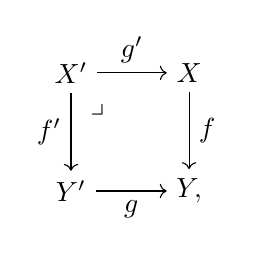
\begin{tikzpicture}[auto,->] 
    \node (tl) at (0,1.5) {$X'$}; 
    \node (tr) at (1.5,1.5) {$X$};
    \node (bl) at (0,0) {$Y'$}; 
    \node (br) at (1.5,0) {$Y,$}; 
    % horizontal lines
    \draw (tl) -- node {$g'$} (tr); 
    \draw (bl) -- node[swap] {$g$} (br); 
    % vertical lines
    \draw (tl) -- node[swap] {$f'$} (bl);
    \draw (tr) -- node {$f$} (br); 
    % pullback symbol (\lrcorner) in the lower right corner of (tl)
    \node at ([xshift=0.0cm, yshift=-0.2cm] tl.south east) {$\lrcorner$};
  \end{tikzpicture}\]
  there exists a natural isomorphism 
  \begin{align*}
    g^{*}f_{!} \simeq f'_{!}g'^{*}
  \end{align*}
  of functors $D(X) \to D(Y')$.
  % \[\begin{tikzpicture}[auto,->] 
  %   \node (tl) at (0,1.5) {$D(X')$}; 
  %   \node (tr) at (2,1.5) {$D(X)$};
  %   \node (bl) at (0,0) {$D(Y')$}; 
  %   \node (br) at (2,0) {$D(Y)$}; 
  %   % horizontal lines
  %   \draw (tr) -- node[swap] {$g'^{*}$} (tl); 
  %   \draw (br) -- node {$g^{*}$} (bl); 
  %   % vertical lines
  %   \draw (tl) -- node[swap] {$f'_{!}$} (bl);
  %   \draw (tr) -- node {$f_{!}$} (br); 
  % \end{tikzpicture}\]
\end{theorem}

\begin{theorem}[Projection Formula] \label{thrm.projection_formula}
  Let $f : X \to Y$ be a proper map of topological spaces.
  Then there exist a natural isomorphism
  \begin{align*}
    f_{!}(-) \otimes (-) \to f_{!}((-) \otimes f^{*}(-))
  \end{align*}
  of functors $D(X) \times D(Y) \to D(Y)$
\end{theorem}

% \begin{theorem}[Projection Formula] \label{thrm.projection_formula}
%   Let $f : X \to Y$ be a proper map of topological spaces, $F$ be a sheaf on $X$, and let $G$ be a sheaf on $Y$.
%   Then the canonical map
%   \begin{align*}
%     f_{!}F \otimes G \to f_{!}(F \otimes f^{*}G)
%   \end{align*}
%   is an isomorphism in $D(Y)$.
% \end{theorem}

% \begin{theorem}[K\"{u}nneth Formula]
%   Let $X$ and $Y$ be topological spaces.
%   Then there exists a natural isomorphism
%   \begin{align*}
%     \bbR\Gamma(X;\bbZ) \otimes \bbR\Gamma(Y;\bbZ) \simeq \bbR\Gamma(X \times Y;\bbZ).
%   \end{align*}
% \end{theorem}


\section{Six-Functor Formalisms} \label{sec.six_functors_formalisms}

From here all categories are assumed to be $\infty$-categories.
In this section, we introduce Mann's definition of six-functor formalisms, considering the following setup:
\begin{itemize}
  \item A category $\C$ of the "geometric objects."
  \item A class $E$ of morphisms in $\C$, where the exceptional functors $f_{!}$ and $f^{!}$ can be defined.
\end{itemize}
For example, this could be the category of sheaves, with the class of morphisms which have finite cohomology dimension.
We assume the following hypothesis (motivated by the above example):
\begin{itemize}
  \item The category $\C$ admits finite limits.
  \item The class $E$ contains all equivalences, and is stable under composition and pullbacks.
\end{itemize}
We expect a six-functor formalism $D$ to satisfy the following conditions (see results in \cref{subsec.remarkable_results}):
\begin{enumerate}
  \item $D$ assigns each object $X$ of $\C$ to a category $D(X)$.
  \item For every object $X$ of $\C$, $D(X)$ is equipped with a symmetric monoidal structure $\otimes$ (\cref{thrm.symmetric_monoidality}).
  \item For every morphism $f : X \to Y$ in $\C$, there is an inverse functor $f^{*} : D(Y) \to D(X)$ which is compatible with composition in $\C$ and with the symmetric monoidal structure (\cref{thrm.symmetric_monoidality,thrm.naturality}).
  \item For every morphism $f : X \to Y$ in $E$, there is an exceptional inverse functor $f_{!} : D(X) \to D(Y)$ which is compatible with composition in $\C$ and satisfies the proper base change theorem and projection formula (\cref{thrm.naturality,thrm.proper_base_change,thrm.projection_formula}).
  \item The functors $\otimes, f^{*}$ and $f_{!}$ admit right adjoint functors $\underline{\Hom}, f_{*}$ and $f^{!}$.
\end{enumerate}
Since there are two morphisms in opposite directions, $f^{*} : D(Y) \to D(X)$ and $f_{!} : D(X) \to D(Y)$, associated with a morphism $f : X \to Y$, it is necessary to define a new category which contains both categories $\C^{\myop}$ and $\C_{E}$.
This new category can be constructed using the \textit{category of correspondences}, denoted $\Corr(\C,E)$.
 
With this setup, conditions (1)-(3) can be encoded by a lax symmetric monoidal functor 
\begin{align*}
  \Corr(\C,E) \to \CMon(\Cat),
\end{align*}
where $\CMon(\Cat)$ is the category of symmetric monoidal categories with symmetric monoidal functors.
Condition (5) is simply a requirement that will be satisfied.
The most difficult part is encoding condition (4).

\subsection{Definitions} \label{subsec.six_functors_formalisms}

In this section, we introduce Mann's definition of six-functor formalisms.
The goal of this section is show the proper base change theorem and projection formula in this setting (\cref{Mann.prop.A.5.8}). 
We first define the geometric setup and give some examples.

\begin{definition}[\cite{Mann22} Definition A.5.1] \label{Mann.def.A.5.1}
  A \textit{geometric setup} $(\C,E)$ consists of the following data:
  \begin{itemize}
    \item A category $\C$ which admits finite limits.
    \footnote{
      In \cite{Mann22}, this condition is not required. 
      However, in many cases, $\C$ satisfies this condition.
      We follow from \cite{Sch22}.
    }
    \item A class $E$ of morphisms in $\C$ which contains all equivalences, and is stable under composition and pullbacks along morphisms in $\C$.
    \footnote{
      In \cite{HM24}, the additional condition is required: 
      for every morphism $X \to Y$ in $E$, the diagonal $X \to X \times_{Y} X$ lies in $E$.
      It is equivalent to the following condition:
      the inclusion $\C_{E} \subseteq \C$ preserves fiber products (\cite{HM24} Lemma 2.1.5).
      This condition is not essential in this note. 
      See \cite{HM24} Remark 2.1.2.
    }
  \end{itemize}
\end{definition}

\begin{notation}
  Let $(\C,E)$ be a geometric setup.
  We let $\C_{E}$ denote the subcategory of $\C$ consisting of the morphisms in $E$.
\end{notation}

\begin{example}
  Let $\C$ be a category which admits finite limits.
  \begin{enumerate}
    \item The pair $(\C,\C)$ is a trivial geometric setup.
    \item The pair $(\C,\core\C)$ is a geometric setup, where $\core\C$ is the underlying anima of $\C$.
    \item If a pair $(\C,E)$ is a geometric setup, then so is the pair $(E,E)$. 
  \end{enumerate}
\end{example}

\begin{definition}[\cite{HA} Construction 5.2.1.1]
  Let $\C$ be a category.
  The \textit{twisted arrow category} $\TwAr(\C)$ of $\C$ is the simplicial set which is defined by 
  \begin{align*}
    \TwAr(\C)_n := \Hom_{\mathrm{sSet}}([n] \star [n]^{\myop},\C)
  \end{align*}
  for every $n \geq 0$, where $\star$ is the join operator.
  By \cite{HA} Proposition 5.2.1.3, $\TwAr(\C)$ is a category.
  A morphism of $\TwAr(\C)$ is called \textit{vertical} (resp. \textit{horizontal}) if its projection to the second (resp. first) factor is degenerate.
\end{definition}

\begin{definition}[\cite{Mann22} Definition A.5.2] \label{Mann.def.A.5.2}
  Let $(\C,E)$ be a geometric setup.
  The \textit{category of correspondences} $\Corr(\C,E)$ is the simplicial set where the $n$-simplices are the functors $X : \TwAr([n]) \to \C$ which satisfy the following conditions:
  \begin{enumerate}
    \item The functor $X$ sends every vertical edge in $\TwAr([n])$ to $E$.
    \item  The functor $X$ sends every biCartesian diagram in $\TwAr([n])$ to a Cartesian diagram in $\C$.
  \end{enumerate}
  By \cite{LZ17} Lemma 6.1.2, $\Corr(\C,E)$ is a category.
\end{definition}

\begin{remark}
  Let $(\C,E)$ be a geometric setup.
  Then the lower simplices of $\Corr(\C,E)$ can be described as follows:
  \begin{itemize}
    \item The objects of $\Corr(\C,E)$ are the objects of $\C$.
    \item A morphism $X \to Y$ in $\Corr(\C,E)$ is given by the following diagram in $\C$
    \[\begin{tikzpicture}[auto,->]
      \node (11) at (0,3) {$X$};
      \node (12) at (1.5,3) {$X'$};
      \node (22) at (1.5,1.5) {$Y,$};
      % horizontal lines
      \draw (12) -- node[swap] {$h$} (11);
      % vertical lines
      \draw (12) -- node {$v$} (22);
    \end{tikzpicture}\]
    where $X'$ is an object of $\C$ and $v$ is a morphism in $E$.
    \item A composition of morphisms $X \to Y$ and $Y \to Z$ in $\Corr(\C,E)$ represented by diagrams $X \xleftarrow{h_1} X' \xrightarrow{v_1} Y$ and $Y \xleftarrow{h_2} Y' \xrightarrow{v_2} Z$ in $\C$ respectively, is given by the following diagram in $\C$.
    \[\begin{tikzpicture}[auto,->]
      \node (11) at (0,3) {$X$};
      \node (12) at (1.5,3) {$X'$};
      \node (13) at (3.5,3) {$X \times_{Y} Y'$};
      \node (22) at (1.5,1.5) {$Y$};
      \node (23) at (3.5,1.5) {$Y'$};
      \node (33) at (3.5,0) {$Z.$};
      % horizontal lines
      \draw (12) -- node[swap] {$h_1$} (11);
      \draw (13) -- node[swap] {} (12);
      \draw (23) -- node[swap] {$h_2$} (22);
      % vertical lines
      \draw (12) -- node {$v_1$} (22);
      \draw (13) -- node {} (23);
      \draw (23) -- node {$v_2$} (33);
      % pullback symbol
      \node at (3.1,2.6) {\rotatebox[origin=c]{90}{$\ulcorner$}};
    \end{tikzpicture}\]  
  \end{itemize}
\end{remark}

\begin{remark}
  Let $(\C,E)$ be a geometric setup.
  We have the canonical inclusions
  \begin{align*}
    \C^{\myop} \subseteq \Corr(\C,E)
  \end{align*}
  defined by mapping $X \xrightarrow{f} Y$ to $Y \xleftarrow{f} X \xrightarrow{\id_X} X$ and 
  \begin{align*}
    \C_E \subseteq \Corr(\C,E)
  \end{align*}
  defined by mapping $X \xrightarrow{f} Y$ to $X \xleftarrow{\id_X} X \xrightarrow{f} Y$.
\end{remark}

\begin{notation}
  Let $\C$ be a category.
  We denote by $\C^{\coprod} \to \Fin_{*}$ the operad described in \cite{HA} Proposition 2.4.3.3.
  Then the fiber $\C^{\coprod}_{\angle{n}}$ is equivalent to $\C^{n}$ for every $n \geq 0$.
\end{notation}

\begin{definition}[\cite{Mann22} Definition A.5.3] \label{Mann.def.A.5.3}
  Let $(\C,E)$ be a geometric setup.
  We define the class $E'$ of morphisms in $(\C^{\myop})^{\coprod,\myop}$ as follows:
  Let $f$ be a morphism in $(\C^{\myop})^{\coprod,\myop}$ which lies over $\alpha : \angle{m} \to \angle{n}$ in $\Fin_{*}$ of the form $(\angle{n}, (Y_j)_{1 \leq j \leq n}) \to (\angle{m}, (X_i)_{1 \leq i \leq m})$.
  Then $E'$ consists of those $f$ for which $\alpha$ is the identity map, and the each induced map $Y_i \to X_i$ belongs to $E$.
\end{definition}

\begin{definition}[\cite{Mann22} Definition A.5.4] \label{Mann.def.A.5.4}
  Let $(\C,E)$ be a geometric setup.
  We denote 
  \begin{align*}
    \Corr(\C,E)^{\otimes} := \Corr((\C^{\myop})^{\coprod,\myop}, E').
  \end{align*}
  According to \cite{LZ17} Lemma 6.1.3, there exists the canonical functor 
  \begin{align*}
    \Corr(\C,E)^{\otimes} \to \Fin_{*}
  \end{align*}
  which endows an operad structure on $\Corr(\C,E)^{\otimes}$ whose underlying category is $\Corr(\C,E)$.
\end{definition}

\begin{remark} \label{Mann.A.5.5}
  Let $\C$ be a category which admits finite products.
  Then $\C$ admits a unique symmetric monoidal structure whose operation is the Cartesian product.
  In particular, the category $\Cat$ admits the product symmetric monoidal structure.
  By \cite{LZ17} Lemma 6.1.3, $\Corr(\C,E)^{\otimes}$ is a symmetric monoidal category.
\end{remark}  

\begin{definition}[\cite{Mann22} Definition A.5.6] \label{Mann.def.A.5.6}
  Let $(\C,E)$ be a geometric setup.
  A \textit{3-functor formalism} on $(\C,E)$ is a lax symmetric monoidal functor
  \begin{align*}
    D : \Corr(\C,E) \to \Cat.
  \end{align*}
  Equivalently, it is a functor 
  \begin{align*}
    D : \Corr(\C,E)^{\otimes} \to \Cat^{\otimes}
  \end{align*}
  such that for every finite set $I$ and a set of objects $(X_i)_{i \in I}$ of $\C$, the functor 
  \begin{align*}
    D(I,(X_i)_{i \in I}) \to \prod_{i \in I} D(X_i)
  \end{align*}
  is an equivalence in $\Cat^{\otimes}$.
\end{definition}

\begin{remark}
  Let $(\C,E)$ be a geometric setup.
  Then the inclusion $(\C^{\myop})^{\coprod,\myop} \subseteq \Corr(\C,E)^{\otimes}$ is a lax symmetric monoidal functor.
  Let $ D : \Corr(\C,E)^{\otimes} \to \Cat^{\otimes}$ be a 3-functor formalism on $(\C,E)$.
  From \cite{HA} Theorem 2.4.3.18, the restriction (it is a lax symmetric monoidal functor)
  \begin{align*}
    D|_{(\C^{\myop})^{\coprod,\myop}} : (\C^{\myop})^{\coprod,\myop} \subseteq \Corr(\C,E)^{\otimes} \to \Cat^{\otimes}
  \end{align*}
  corresponds to a functor 
  \begin{align*}
    D^{*} : \C^{\myop} \to \CMon(\Cat).
  \end{align*}
  By the restriction, we obtain a functor 
  \begin{align*}
    D_{!} := D|_{\C_{E}} : \C_{E} \subseteq \Corr(\C,E) \to \Cat.
  \end{align*}
\end{remark}

\begin{notation}
  Let $(\C,E)$ be a geometric setup, and let $ D : \Corr(\C,E)^{\otimes} \to \Cat^{\otimes}$ be a 3-functor formalism on $(\C,E)$.
  We will use the following notations:
  \begin{enumerate}
    \item For every object $X$ of $\C$, the category $D(X)=D^{*}(X)$ admit a symmetric monoidal structure, which we denote by 
    \begin{align*}
      \otimes : D(X) \times D(X) \to D(X).
    \end{align*}
    \item For every morphism $f : X \to Y$ in $\C$, we obtain a symmetric monoidal functor 
    \begin{align*}
      f^{*} := D^{\ast}(f) : D(Y) \to D(X).
    \end{align*}
    \item For every morphism $f : X \to Y$ in $E$, we obtain a functor
    \begin{align*}
      f_{!} := D_{!}(f) : D(X) \to D(Y).
    \end{align*}
  \end{enumerate}
\end{notation}

\begin{definition}[\cite{Mann22} Definition A.5.7] \label{Mann.def.A.5.7}
  Let $(\C,E)$ be a geometric setup.
  A \textit{6-functor formalism} on $(\C,E)$ is a 3-functor formalism $ D : \Corr(\C,E)^{\otimes} \to \Cat^{\otimes}$ on $(\C,E)$ which satisfies the following conditions:
  \begin{enumerate}
    \item For every object $X$ of $\C$, the symmetric monoidal structure on $D(X)$ is closed.
    \item The functors $f^{*} : D(Y) \to D(X)$ and $f_! : D(X) \to D(Y)$ admit right adjoint functors.
  \end{enumerate}
\end{definition}

\begin{notation}
  Let $(\C,E)$ be a geometric setup, and let $D : \Corr(\C,E)^{\otimes} \to \Cat^{\otimes}$ be a 6-functor formalism on $(\C,E)$.
  We will use the following notations:
  \begin{enumerate}
    \item We denote the internal hom in $D(X)$ (i.e. the right adjoint functor to $\otimes$) by 
    \begin{align*}
      \underline{\Hom} : D(X)^{\myop} \times D(X) \to D(X).
    \end{align*}
    \item For every morphism $f : X \to Y$ in $\C$, we denote the right adjoint functor to $f^{*}$ by 
    \begin{align*}
      f_{*} : D(X) \to D(Y).
    \end{align*}
    We denote by $D_{*} : \C \to \Cat$ determined by the constructions $X \mapsto D(X)$ and $f \mapsto f_{*}$.
    \item For every morphism $f : X \to Y$ in $E$, we denote the right adjoint functor to $f_{!}$ by 
    \begin{align*}
      f^{!} : D(Y) \to D(X).
    \end{align*}
    We denote by $D^{!} : \C_{E}^{\myop} \to \Cat$ determined by the constructions $X \mapsto D(X)$ and $f \mapsto f^{!}$.
  \end{enumerate}
\end{notation}

\begin{proposition}[\cite{Mann22} Proposition A.5.8] \label{Mann.prop.A.5.8}
  Let $(\C,E)$ be a geometric setup, and let $ D : \Corr(\C,E)^{\otimes} \to \Cat^{\otimes}$ be a 6-functor formalism on $(\C,E)$.
  Then the associated six functors $\otimes, \underline{\Hom}, f^{*}, f_{*}, f_{!}$ and $f^{!}$ satisfy the following conditions:
  \begin{enumerate}
    \item The functors $f^{*}, f_{\ast}, f_{!}$ and $f^{!}$ are compatible with composition.
    \item For every morphism $f : X \to Y$ in $\C$, the functor $f^{*} : D(Y) \to D(X)$ is symmetric monoidal.
    \item (Proper Base Change) For every Cartesian diagram in $\C$ 
    \[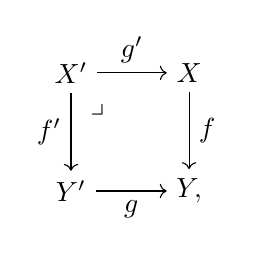
\begin{tikzpicture}[auto,->] 
      \node (tl) at (0,1.5) {$X'$}; 
      \node (tr) at (1.5,1.5) {$X$};
      \node (bl) at (0,0) {$Y'$}; 
      \node (br) at (1.5,0) {$Y,$}; 
      % horizontal lines
      \draw (tl) -- node {$g'$} (tr); 
      \draw (bl) -- node[swap] {$g$} (br); 
      % vertical lines
      \draw (tl) -- node[swap] {$f'$} (bl);
      \draw (tr) -- node {$f$} (br); 
      % pullback symbol (\lrcorner) in the lower right corner of (tl)
      \node at ([xshift=0.0cm, yshift=-0.2cm] tl.south east) {$\lrcorner$};
    \end{tikzpicture}\]
    where $f$ in $E$ (thus also $f'$ in $E$), there exists a natural equivalence
    \begin{align*}
      g^{*}f_{!} \simeq f'_{!}g'^{*}
    \end{align*}
    of functors $D(X) \to D(Y')$.
    \[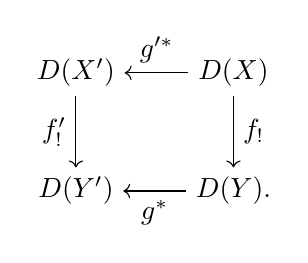
\begin{tikzpicture}[auto,->] 
      \node (tl) at (0,1.5) {$D(X')$}; 
      \node (tr) at (2,1.5) {$D(X)$};
      \node (bl) at (0,0) {$D(Y')$}; 
      \node (br) at (2,0) {$D(Y).$}; 
      % horizontal lines
      \draw (tr) -- node[swap] {$g'^{*}$} (tl); 
      \draw (br) -- node {$g^{*}$} (bl); 
      % vertical lines
      \draw (tl) -- node[swap] {$f'_{!}$} (bl);
      \draw (tr) -- node {$f_{!}$} (br); 
    \end{tikzpicture}\]
    \item (Projection Formula) For every morphism $f : X \to Y$ in $E$,
    there exists a natural equivalence
    \begin{align*}
      f_{!}(-) \otimes (-) \to f_{!}((-) \otimes f^{*}(-))
    \end{align*}
    of functors $D(X) \times D(Y) \to D(Y)$.
    \[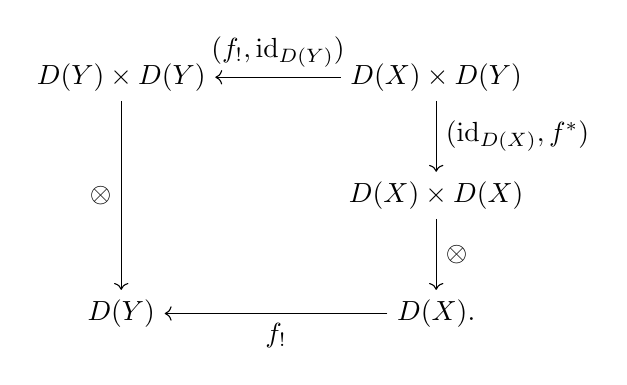
\begin{tikzpicture}[auto,->] 
      \node (tl) at (0,3) {$D(Y) \times D(Y)$}; 
      \node (tr) at (4,3) {$D(X) \times D(Y)$};
      \node (mr) at (4,1.5) {$D(X) \times D(X)$};
      \node (bl) at (0,0) {$D(Y)$}; 
      \node (br) at (4,0) {$D(X).$}; 
      % horizontal lines
      \draw (tr) -- node[swap] {$(f_!,\id_{D(Y)})$} (tl); 
      \draw (br) -- node {$f_{!}$} (bl); 
      % vertical lines
      \draw (tl) -- node[swap] {$\otimes$} (bl);
      \draw (tr) -- node {$(\id_{D(X)},f^{*})$} (mr);
      \draw (mr) -- node {$\otimes$} (br); 
    \end{tikzpicture}\]
  \end{enumerate}
\end{proposition}

\begin{proof}
  (1) and (2) follow from the definitions.

  The morphisms $f : X \to Y$ in $E$ and $g : Y' \to Y$ in $\C$ determine correspondences $h_1$ and $h_2$ respectively.
  \[\begin{tikzpicture}[auto]
    \node (11) at (0,1.5) {$X$};
    \node (12) at (1.5,1.5) {$X$};
    \node (13) at (3,1.5) {$Y$};
    \node (14) at (4.5,1.5) {$Y'$};
    \node (22) at (1.5,0) {$Y$};
    \node (24) at (4.5,0) {$Y'.$};
    % horizontal lines
    \draw[transform canvas={yshift=1.5pt}] (12) -- (11);
    \draw[transform canvas={yshift=-1.5pt}] (12) -- (11);   
    \draw[->] (14) -- node[swap] {$g$} (13);
    % vertical lines
    \draw[->] (12) -- node {$f$} (22);
    \draw[transform canvas={xshift=1.5pt}] (14) -- (24);
    \draw[transform canvas={xshift=-1.5pt}] (14) -- (24);
  \end{tikzpicture}\]

  The composition $h_1h_2$ is given by the correspondence
  \[\begin{tikzpicture}[auto]
    \node (11) at (0,3) {$X$};
    \node (12) at (1.5,3) {$X$};
    \node (13) at (3,3) {$X'$};
    \node (22) at (1.5,1.5) {$Y$};
    \node (23) at (3,1.5) {$Y'$};
    \node (33) at (3,0) {$Y'.$};
    % horizontal lines
    \draw[transform canvas={yshift=1.5pt}] (12) -- (11);
    \draw[transform canvas={yshift=-1.5pt}] (12) -- (11);   
    \draw[->] (13) -- node[swap] {$g'$} (12);
    \draw[->] (23) -- node[swap] {$g$} (22);
    % vertical lines
    \draw[->] (12) -- node {$f$} (22);
    \draw[->] (13) -- node {$f'$} (23);
    \draw[transform canvas={xshift=1.5pt}] (23) -- (33);
    \draw[transform canvas={xshift=-1.5pt}] (23) -- (33);
    % pullback symbol
    \node at (2.6,2.6) {\rotatebox[origin=c]{90}{$\ulcorner$}};
  \end{tikzpicture}\]
  The first map $h_1 : X \xleftarrow{\id_X} X \xrightarrow{f} Y$ defines a functor 
  \begin{align*}
    f_! : D(X) \to D(Y).
  \end{align*}
  The second map $h_2 : Y \xleftarrow{g'} Y' \xrightarrow{\id_Y} Y'$ defines a functor 
  \begin{align*}
    g^{*} : D(Y) \to D(Y').
  \end{align*}
  The composition $h_1h_2 : X \xleftarrow{g'} X' \xrightarrow{f'} Y'$ defines a functor
  \begin{align*}
    f'_{!}g'^{*} : D(X) \to D(Y').
  \end{align*}
  Thus we obtain a natural equivalence $g^{*}f_{!} \simeq f'_{!}g'^{*}$, since $D$ is a functor.

  We finally show (4).
  Let $f : X \to Y$ be a morphism in $E$.
  We consider the map $X \times Y \to Y$ given by the correspondence
  \[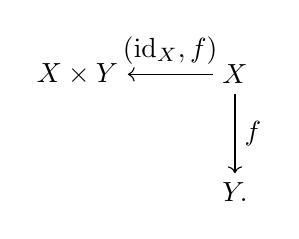
\begin{tikzpicture}[auto,->]
    \node (11) at (-0.5,3) {$X \times Y$};
    \node (12) at (1.5,3) {$X$};
    \node (22) at (1.5,1.5) {$Y.$};
    % horizontal lines
    \draw (12) -- node[swap] {$(\id_X,f)$} (11);
    % vertical lines
    \draw (12) -- node {$f$} (22);
  \end{tikzpicture}\]
  We obtain its two factorizations as follows:
  The map $X \times Y \to Y \times Y \to Y$ which is given by the correspondence
  \[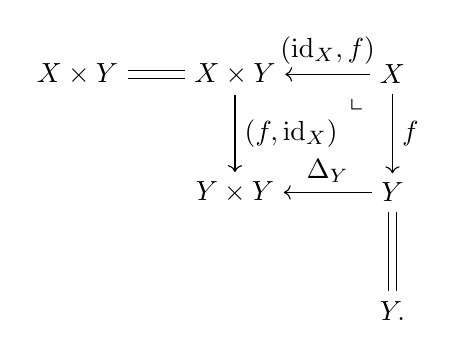
\begin{tikzpicture}[auto]
    \node (11) at (-0.5,3) {$X \times Y$};
    \node (12) at (1.5,3) {$X \times Y$};
    \node (13) at (3.5,3) {$X$};
    \node (22) at (1.5,1.5) {$Y \times Y$};
    \node (23) at (3.5,1.5) {$Y$};
    \node (33) at (3.5,0) {$Y.$};
    % horizontal lines
    \draw[transform canvas={yshift=1.5pt}] (12) -- (11);
    \draw[transform canvas={yshift=-1.5pt}] (12) -- (11);
    \draw[->] (13) -- node[swap] {$(\id_X,f)$} (12);
    \draw[->] (23) -- node[swap]{$\Delta_Y$} (22);
    % vertical lines
    \draw[->] (12) -- node {$(f,\id_X)$} (22);
    \draw[->] (13) -- node {$f$} (23);
    \draw[transform canvas={xshift=1.5pt}] (23) -- (33);
    \draw[transform canvas={xshift=-1.5pt}] (23) -- (33);
    % pullback symbol
    \node at (3.1,2.6) {\rotatebox[origin=c]{90}{$\ulcorner$}};
  \end{tikzpicture}\]
  The map $X \times Y \to X \times X \to X \to Y$ which is given by the correspondence
  \[\begin{tikzpicture}[auto]
    \node (11) at (-1.5,4.5) {$X \times Y$};
    \node (12) at (1.0,4.5) {$X \times X$};
    \node (13) at (3,4.5) {$X$};
    \node (14) at (4.5,4.5) {$X$};
    \node (22) at (1.0,3) {$X \times X$};
    \node (23) at (3,3) {$X$};
    \node (24) at (4.5,3) {$X$};
    \node (33) at (3,1.5) {$X$};
    \node (34) at (4.5,1.5) {$X$};
    \node (44) at (4.5,0) {$Y.$};
    % horizontal lines
    \draw[->] (12) -- node[swap] {$(\id_X,f)$} (11);
    \draw[->] (13) -- node[swap] {$\Delta_X$} (12);
    \draw[transform canvas={yshift=1.5pt}] (14) -- (13);
    \draw[transform canvas={yshift=-1.5pt}] (14) -- (13);   
    \draw[->] (23) -- node[swap] {$\Delta_X$} (22);
    \draw[transform canvas={yshift=1.5pt}] (24) -- (23);
    \draw[transform canvas={yshift=-1.5pt}] (24) -- (23);  
    \draw[transform canvas={yshift=1.5pt}] (34) -- (33);
    \draw[transform canvas={yshift=-1.5pt}] (34) -- (33);  
    % vertical lines
    \draw[transform canvas={xshift=1.5pt}] (12) -- (22);
    \draw[transform canvas={xshift=-1.5pt}] (12) -- (22);
    \draw[transform canvas={xshift=1.5pt}] (13) -- (23);
    \draw[transform canvas={xshift=-1.5pt}] (13) -- (23);
    \draw[transform canvas={xshift=1.5pt}] (23) -- (33);
    \draw[transform canvas={xshift=-1.5pt}] (23) -- (33);
    \draw[transform canvas={xshift=1.5pt}] (14) -- (24);
    \draw[transform canvas={xshift=-1.5pt}] (14) -- (24);
    \draw[transform canvas={xshift=1.5pt}] (24) -- (34);
    \draw[transform canvas={xshift=-1.5pt}] (24) -- (34);
    \draw[transform canvas={xshift=1.5pt}] (34) -- (34);
    \draw[transform canvas={xshift=-1.5pt}] (34) -- (34);
    \draw[->] (34) -- node {$f$} (44);
    % pullback symbol
    \node at (2.6,4.1) {\rotatebox[origin=c]{90}{$\ulcorner$}};
    \node at (4.1,4.1) {\rotatebox[origin=c]{90}{$\ulcorner$}};
    \node at (4.1,2.6) {\rotatebox[origin=c]{90}{$\ulcorner$}};
  \end{tikzpicture}\]
  The map $X \times Y \xleftarrow{(\id_X,f)} X \xrightarrow{f} Y$ defines a functor 
  \begin{align*}
    D(X) \times D(Y) \to D(Y).
  \end{align*}
  The first factorization $X \times Y \xleftarrow{(\id_X,f)} X \xrightarrow{f} Y$ defines a functor
  \begin{align*}
    D(X) \times D(Y) \to D(Y) \times D(Y) \to D(Y) 
    : (F,G) \to (f_{!}F, G) \mapsto f_{!}F \otimes G.
  \end{align*}
  The second factorization $X \times Y \xleftarrow{(\id_X,f)} X \times X \xleftarrow{\Delta_X} X \xrightarrow{f} Y$ defines a functor 
  \begin{align*}
    D(X) \times D(Y) \to D(X) \times D(X) \to D(X) \to D(Y) 
    : (F,G) \mapsto (F,f^{*}G) \mapsto F \otimes f^{*}G \mapsto f_!(F \otimes f^{*}G).
  \end{align*}
  This implies that a map $f_{!}F \otimes G \to f_!(F \otimes f^{*}G)$ is an equivalence in $D(Y)$, since $D$ is a functor.
\end{proof} 

\subsection{With Suitable Decompositions} \label{subsec.with_suitable_decompositions}

In practice, there are two special subclasses of morphisms $I$ and $P$ of $E$ of "open immersions" and "proper maps", which satisfies the following conditions:
\begin{enumerate}
  \item For every morphism $f$ in $I$, $f_{!}$ is left adjoint to $f^{*}$. i.e. $f_! \dashv f^{*}$.
  \item For every morphism $f$ in $P$, $f_{!}$ is right adjoint to $f^{*}$. i.e. $f^{*} \dashv f_!$ and $f_{!} = f_{*}$.
  \item Every morphism $f$ in $E$ admits a factorization $f=\overline{f}j$, where $j$ in $I$ and $\overline{f}$ in $P$. 
  \item The functor $f_{!}$ is compatible with the above factorization. i.e. $f_{!} = \overline{f}_{!}j_{!}$.
\end{enumerate}

\begin{example} \label{Sch.eg.4.1}
  Let $\C$ be the category of locally compact Hausdorff topological spaces, and $E$ be the class of all morphisms.
  Let $I$ and $P$ be the classes of open immersions and proper maps, respectively.
  Then every morphism $f$ in $E (= \C)$ admits a factorization $X \xrightarrow{j} \overline{X} \xrightarrow{\overline{f}} Y$, where $j$ in $I$ and $\overline{f}$ in $P$.
  For example, we can choose $\overline{X} = \beta X \times_{\beta Y} Y$ using the Stone-\v{C}ech compactification. 
\end{example}

However, it is not obvious that $f_{!}$ is well-defined i.e. $f_{!}$ is independent on the choice of the factorization and it satisfies the required compatibilities for 6-functor formalisms.
We need the following conditions to make the above construction work.

\begin{definition}[\cite{Mann22} Definition A.5.9] \label{Mann.def.A.5.9}
  Let $(\C,E)$ be a geometric setup.
  We will say that $E$ \textit{has a suitable decomposition} $(I,P)$ if there exists a pair of subclasses of morphisms $(I,P)$ of $E$ which satisfies the following conditions:
  \begin{enumerate}
    \item The classes $I$ and $P$ contain all equivalences, and are stable under composition and pullbacks.
    \item Every morphism $f$ in $E$ admits a factorization $f=\overline{f}j$, where $j$ in $I$ and $\overline{f}$ in $P$.
    \item Let $f : X \to Y$ and $g : Y \to Z$ be morphisms in $\C$.
    If $g$ is in $I$ (resp. $g$ in $P$), then $f$ is in $I$ (resp. $f$ in $P$) if and only if $gf$ is in $I$ (resp. $gf$ in $P$).
    \item Every morphism $f$ in $I \cap P$ is $n$-truncated for some $n > -2$ (which may depend on $f$).
  \end{enumerate}
\end{definition}

\begin{definition}
  Let $(\C,E)$ be a geometric setup, and let $D^{*} : \C^{\myop} \to \CMon(\Cat)$ be a functor.
  Suppose that $E$ has a suitable decomposition $(I,P)$.
  For every morphism $f : X \to Y$ in $\C$, we denote $f^{*} := D^{*}(f) : D^{*}(Y) \to D^{*}(X)$.
  We will say that $D^{*}$ \textit{satisfies a suitable decomposition condition} for $(I,P)$ if it satisfies the following conditions:
  \begin{enumerate}
    \item For every morphism $j$ in $I$, the functor $j^{*}$ admits a left adjoint functor $j_{!}$, which satisfies the proper base change and (proper) projection formula.
    \item For every morphism $g$ in $P$, the functor $g^{*}$ admits a right adjoint functor $g_{*}$, which satisfies the $*$-version base change and $*$-version projection formula.
    \item For every Cartesian diagram in $\C$
    \[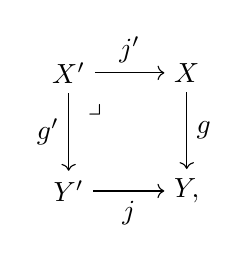
\begin{tikzpicture}[auto,->] 
      \node (tl) at (0,1.5) {$X'$}; 
      \node (tr) at (1.5,1.5) {$X$};
      \node (bl) at (0,0) {$Y'$}; 
      \node (br) at (1.5,0) {$Y,$}; 
      % horizontal lines
      \draw (tl) -- node {$j'$} (tr); 
      \draw (bl) -- node[swap] {$j$} (br); 
      % vertical lines
      \draw (tl) -- node[swap] {$g'$} (bl);
      \draw (tr) -- node {$g$} (br); 
      % pullback symbol (\lrcorner) in the lower right corner of (tl)
      \node at ([xshift=0.0cm, yshift=-0.2cm] tl.south east) {$\lrcorner$};
    \end{tikzpicture}\]
    where $j$ in $I$ (thus also $j'$ in $I$), and $g$ in $P$ (thus also $g'$ in $P$), there exists a natural equivalence
    \begin{align*}
      j_{!}g'_{*} \to g_{*}j'_{!}
    \end{align*}
    of functors $D^{*}(X') \to D^{*}(Y)$.
    \[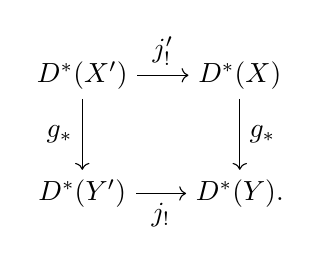
\begin{tikzpicture}[auto,->] 
      \node (tl) at (0,1.5) {$D^{*}(X')$}; 
      \node (tr) at (2,1.5) {$D^{*}(X)$};
      \node (bl) at (0,0) {$D^{*}(Y')$}; 
      \node (br) at (2,0) {$D^{*}(Y).$}; 
      % horizontal lines
      \draw (tl) -- node {$j'_{!}$} (tr); 
      \draw (bl) -- node[swap] {$j_{!}$} (br); 
      % vertical lines
      \draw (tl) -- node[swap] {$g_{*}$} (bl);
      \draw (tr) -- node {$g_{*}$} (br); 
    \end{tikzpicture}\]
  \end{enumerate}
\end{definition}

\begin{proposition}[\cite{Mann22} Proposition A.5.10] \label{Mann.prop.A.5.10}
  Let $(\C,E)$ be a geometric setup.
  Suppose that $E$ has a suitable decomposition $(I,P)$.
  Let $D^{*} : \C^{\myop} \to \CMon(\Cat)$ be a functor which satisfies a suitable decomposition condition for $(I,P)$.
  Then $D^{*}$ can be extended to a 3-functor formalism 
  \begin{align*}
    D : \Corr(\C,E)^{\otimes} \to \Cat^{\otimes},
  \end{align*}
  on $(\C,E)$ such that for every morphism $j$ in $I$, $j_{!}$ is left adjoint to $j^{*}$, and for every morphism $g$ in $P$, $g_{!}$ is right adjoint to $g^{*}$.

  Suppose additionally that $D$ satisfies the following conditions:
  \begin{enumerate}
    \item For every object $X$ of $\C$, the symmetric monoidal structure on $D(X)$ is closed.
    \item For every morphism $f : X \to Y$ in $\C$, the functor $f^{*} : D(Y) \to D(X)$ admit a right adjoint functor $f_{*} : D(X) \to D(Y)$.
    \item For every morphism $g : X \to Y$ in $P$, the functor $f_{*}=f_{!} : D(X) \to D(Y)$ admit a right adjoint functor $f^{!} : D(Y) \to D(X)$.
  \end{enumerate}
  Then the above 3-functor formalism $D$ is a 6-functor formalism on $(\C,E)$. 
\end{proposition}

\appendix 


\section{Derived Categories and Derived Functors} \label{sec.derived_categories}

\subsection{Derived Categories and Derived Functors}

We recall the classical notions of derived categories and (right) derived functors.

\begin{notation}
  Let $\A$ be an abelian category.
  We let
  \begin{itemize}
    \item $C(\A)$ denote the category of complexes of $\A$.
    \item $K(\A)$ denote the homotopy category of complexes of $\A$.
    \item $D(\A)$ denote the derived category of complexes of $\A$.
    % \item $D(\A)$ denote the localization of $K(\A)$ with respect to the set of quasi-isomorphisms, refer to it as the \textit{derived category} of $\A$.
  \end{itemize}
  Let $F : \A \to \B$ be a functor between abelian categories.
  We also denote by $F : K(\A) \to K(\B)$ the induced functor between homotopy categories.
\end{notation}

Let $\A$ and $\B$ be abelian categories.
If a functor $F : K(\A) \to K(\B)$ between homotopy categories is exact, then it preserves quasi-isomorphisms.
In this case, it induces a functor $F : D(\A) \to D(\B)$ between derived categories.
However, in general, it does not necessarily preserves quasi-isomorphisms.
That is, it does not send objects which are isomorphic in $D(\A)$ to objects which are isomorphic in $D(\B)$.
To avoid this issue, we consider derived functors.

\begin{definition}
  Let $F : \A \to \B$ be a left exact functor between abelian categories.
  A \textit{right derived functor} $(\bbR F,\tau)$ is the left Kan extension of $Q_{\B}F$ along $Q_{\A}$.
  \[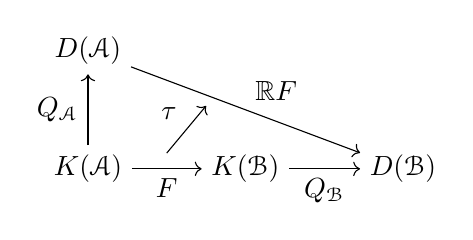
\begin{tikzpicture}[auto,->] 
    \node (tl) at (0,1.5) {$D(\A)$}; 
    \node (bl) at (0,0) {$K(\A)$}; 
    \node (bm) at (2,0) {$K(\B)$};
    \node (br) at (4,0) {$D(\B)$}; 
    % horizontal line 
    \draw (bl) -- node[swap] {$F$} (bm); 
    \draw (bm) -- node[swap] {$Q_{\B}$} (br);
    % vertical line
    \draw (bl) -- node {$Q_{\A}$} (tl);
    % from tl to br
    \draw (tl) -- node {$\bbR F$} (br); 
    \draw (1,0.2) -- node {$\tau$} (1.5,0.8);
  \end{tikzpicture}\]
\end{definition}

We consider the conditions under which derived functors exist.

\begin{definition} \label{Ike.2.1.26}
  Let $F : \A \to \B$ be a left exact functor between abelian categories, and let $\I$ be an additive full subcategory of $\A$.
  We will say that $\I$ is \textit{$F$-injective} if it satisfies the following conditions:
  \begin{enumerate}
    \item For every object $A$ of $\A$, there exist an object $I$ of $\I$ and a monomorphism $A \to I$.
    \item Let $0 \to A \to B \to C \to 0$ is a short exact sequence in $\A$. 
    If $A$ and $B$ are in $\I$, then $C$ is also in $\I$.
    \item Let $0 \to A \to B \to C \to 0$ is a short exact sequence in $\A$.
    If $A$ is in $\I$, then $0 \to F(A) \to F(B) \to F(C) \to 0$ is a short exact sequence in $\B$.
  \end{enumerate}
\end{definition}

\begin{proposition} \label{Ike.2.1.28}
  Let $F : \A \to \B$ be a left exact functor between abelian categories.
  Suppose that there exists an $F$-injective additive full subcategory $\I$ of $\A$.
  Then there exists the right derived functor $\bbR F : D(\A) \to D(\B)$ of $F$.
  Moreover, $\bbR F$ preserves quasi-isomorphisms.
\end{proposition}

\begin{remark} \label{Ike.2.1.30}
  Let $F : \A \to \B$ be a left exact functor between abelian categories.
  If $\A$ has enough injectives, then the additive full subcategory spanned by injective objects of $\A$ is $F$-injective.
  Moreover, there exists the right derived functor $\bbR F : D(\A) \to D(\B)$ of $F$.
\end{remark}

We consider when the derived functor of a composition of two functors is itself a derived functor.

\begin{proposition} \label{Ike.2.1.31}
  Let $F : \A \to \B$ and $G : \B \to \C$ be left exact functors between abelian categories.
  Suppose that there exist an $F$-injective additive full subcategory $\I_{\A}$ of $\A$ and a $G$-injective additive full subcategory $\I_{\B}$ of $\B$ which satisfy $F(\I_{\A}) \subseteq \I_{\B}$.
  Then $\I_{\A}$ is $GF$-injective and there exists a natural isomorphism $\bbR(G \circ F) \simeq \bbR G \circ \bbR F$.
\end{proposition}

We consider the derived category of sheaves and the right derived functor of the global section functor.

\begin{notation} \label{Ike.2.2.2}
  Let $X$ be a topological space.
  We let $D(X)$ denote the derived category of sheaves on $X$.
\end{notation}

\begin{example} 
  Let $X$ be a topological space, and let $\Gamma(X;-) : \Shv(X) \to \Ab$ be the global section functor.
  Then an additive full subcategory of $\Shv(X)$ spanned by flabby sheaves is $\Gamma(X;-)$-injective.
  Thus there exists the right derived functor 
  \begin{align*}
    \bbR \Gamma(X;-) : D(X) \to D(\Ab).
  \end{align*}
  of the global section functor $\Gamma(X;-) : \Shv(X) \to \Ab$.
\end{example}

% In the rest of this section, we discuss the right derived functor of hom functor.

\subsection{Flabby, C-soft, and Flat Sheaves}

In this section, we recall the notions of flabby, c-soft, and flat sheaves.

\begin{definition} \label{Ike.1.2.1}
  Let $X$ be a topological space.
  A sheaf $F$ on $X$ is called \textit{flabby} (or \textit{flasque}) if, for every open subset $U$ of $X$, a morphism $F(X) \to F(U)$ is surjective.
\end{definition}

\begin{proposition}
  Let $X$ be a topological space.
  Then for every sheaf $F$ on $X$, there exist a flabby sheaf $[F]$ and a mono morphism $F \to [F]$.
\end{proposition}

\begin{proposition}
  Let $0 \to F \to G \to H \to 0$ be an exact sequence of sheaves.
  If $F$ is flabby, then the global section functor $\Gamma(X;F) : \Shv(X) \to \Ab$ is exact.
  Moreover, if $F$ and $G$ are flabby, then so is $H$.  
\end{proposition}

\begin{definition} \label{Ike.2.2.12}
  Let $X$ be a topological space.
  A sheaf $F$ on $X$ is called \textit{c-soft} if, for every compact subset $K$ of $X$, a morphism $\Gamma(X;F) \to \Gamma(K,F_{K})$ is surjective.
\end{definition}

\begin{proposition}
  Let $f : X \to Y$ be a continuous map of locally compact Hausdorff spaces.
  Then the full subcategory of $\Shv(X)$ spanned by c-soft sheaves is $f_{!}$-injective.
\end{proposition}

\begin{definition} \label{Ike.2.2.4}
  Let $X$ be a topological space.
  A sheaf $F$ on $X$ is called \textit{flat} if the tensor product functor $F \otimes - : \Shv(X) \to \Shv(X)$ is exact.
\end{definition}

\begin{proposition}
  Let $X$ be a topological space.
  Then for every sheaf $F$ on $X$, there exist a flat sheaf $P$ and an epimorphism $P \to F$.
\end{proposition}

\printbibliography

\end{document}

% \subsection{Extension of Six-Functor Formalisms (TBA)} \label{subsec.extension_of_six_functors_formalisms} 

% We can construct various 6-functor formalisms using \cref{Mann.prop.A.5.10}.
% However, the factorization condition for $(I,P)$ of $E$ is a little strong.
% In this section, we introduce the extension theorems for geometric setups.

% \begin{lemma}[\cite{Mann22} Lemma A.5.11] \label{Mann.lem.A.5.11}
%   Let $(\C,E)$ and $(\C,E')$ be two setups which satisfy $E \subseteq E'$.
%   Let $D : \Corr(\C,E) \to \Cat$ be a 6-functor formalism on $(\C,E)$ which satisfies the following conditions:
%   \begin{enumerate}
%     \item For every object $X$ of $\C$, the category $D(X)$ is presentable.
%     \item For every morphism $f : X \to Y$ in $E$, we let $\I_{f}$ denote the subcategory of $\C_{/X}$ whose objects are the morphisms $g : Z \to X$ such that $g$ and $fg$ are in $E$, and whose morphisms are the morphisms $Z' \to Z$ over $X$ which lies in $E$.
%     For every morphism in $\I_{f}$, the canonical functor 
%     \begin{align*}
%       D^{!}(X) \to \lim_{Z \in \I_{f}^{\myop}} D^{!}(X)
%     \end{align*}
%     is an equivalence.
%   \end{enumerate}
%   Then $D$ can be a 6-functor formalism
%   \begin{align*}
%     D : \Corr(\C,E') \to \Cat
%   \end{align*}
%   on $(\C,E')$.
% \end{lemma}

% \subsection{Poincar\'{e} Duality (TBA)}

% Poincar\'{e} duality implies that for a "smooth" map $f$, the right adjoint functor $f^{!}$ of $f_{!}$ exists and agree with $f^{*}$ up to a twist.
% In this section, we consider this situation in the setting of six-functor formalisms.

% \begin{definition}
%   Let $(\C,E)$ be a geometric setup, and $D : \Corr(\C,E) \to \Cat$ be a 3-functor formalism on $(\C,E)$.
%   A morphism $f : X \to Y$ in $E$ is called ($D$-)\textit{cohomologically smooth} if it satisfies the following conditions:
%   \begin{enumerate}
%     \item 
%   \end{enumerate}
% \end{definition}

% \subsection{Classical Poincar\'{e} Duality (TBA)} \label{subsec.poincare_duality}

% \begin{theorem}[Poincar\'{e} duality for compact oriented manifolds] \label{Hoy.thrm.1.1}
%   (TBA)
% \end{theorem}

% \subsection{Sheaf Cohomology}

% \begin{definition}
%   Let $\A$ be an abelian category which has enough injectives, and let $F : \A \to \B$ be a left exact functor between abelian categories.
%   For every object $A$ of $\A$, we take an injective resolution $0 \to A \to I_A$.
%   Then we obtain a complex in $\B$ by applying $F$ to the complex $I_A$
%   \begin{align*}
%     F(I_A) : F(I_A^0) \xrightarrow{T(d^0)} F(I_A^1) \xrightarrow{T(d^1)} F(I_A^2) \xrightarrow{T(d^2)} \cdots.
%   \end{align*}
%   We define 
%   \begin{align*}
%     R^nF(A) := H^n F(I_A) := \Ker F(d^n) / \Im F(d^{n-1}),
%   \end{align*}
%   which induces a functor 
%   \begin{align*}
%     R^nF : \A \to \B,
%   \end{align*}
%   since the construction $A \mapsto H^nF(I_A)$ is functional on $A$.
%   We will refer to it as the \textit{$n$-th right derived functor} of $F$.
% \end{definition}

% We apply the $n$-th right derived functor for the global section functor.

% \begin{example}
%   Let $X$ be a topological space, and let $\Gamma(X;-) : \Shv(X) \to \Ab$ be the global section functor.
%   Then the \textit{$n$-th sheaf cohomology} 
%   \begin{align*}
%     H^n(X;-) : \Shv(X) \to \Ab
%   \end{align*}
%   is defined as the $n$-th right derived functor $R^n \Gamma(X;-)$ of $\Gamma(X;-)$.
% \end{example}

% By construction, we have 
% \begin{align*}
%   H^n \circ \bbR \Gamma(X;-) = H^n(X;-).
% \end{align*}
% This implies that sheaf cohomology can be lifted to a functor between derived categories.
% \[\begin{tikzpicture}[auto,->] 
%   \node (tl) at (0,1.5) {$D(X)$}; 
%   \node (bl) at (0,0) {$K(\Shv(X))$}; 
%   \node (bm) at (3,0) {$K(\Ab)$};
%   \node (br) at (5,0) {$D(\Ab)$}; 
%   \node (brr) at (7,0) {$\Ab$};
%   % horizontal line 
%   \draw (bl) -- node[swap] {$\Gamma(X;-)$} (bm); 
%   \draw (bm) -- node[swap] {$Q_{\B}$} (br);
%   \draw (br) -- node[swap] {$H^n$} (brr);
%   % vertical line
%   \draw (bl) -- node {$Q_{\A}$} (tl);
%   % from tl to br/brr
%   \draw (tl) -- node {$\bbR \Gamma(X;-)$} (br); 
%   \draw (tl) to[bend left=20] node[pos=0.8] {$H^n(X;-)=R^n\Gamma(X;-)$} (brr); 
% \end{tikzpicture}\]

% We show (3).
% We consider the map $X \xrightarrow{h} Y'$ given by the correspondence
% \[\begin{tikzpicture}[auto,->]
%   \node (11) at (0,3) {$X$};
%   \node (12) at (1.5,3) {$X'$};
%   \node (22) at (1.5,1.5) {$Y'.$};
%   % horizontal lines
%   \draw (12) -- node[swap] {$g'$} (11);
%   % vertical lines
%   \draw (12) -- node {$f'$} (22);
% \end{tikzpicture}\]
% We obtain its factorization as follows:
% The map $X \xrightarrow{h_1} Y \xrightarrow{h_2} Y'$ which is given be the correspondence
% \[\begin{tikzpicture}[auto]
%   \node (11) at (0,3) {$X$};
%   \node (12) at (1.5,3) {$X$};
%   \node (13) at (3,3) {$X'$};
%   \node (22) at (1.5,1.5) {$Y$};
%   \node (23) at (3,1.5) {$Y'$};
%   \node (33) at (3,0) {$Y'.$};
%   % horizontal lines
%   \draw[transform canvas={yshift=1.5pt}] (12) -- (11);
%   \draw[transform canvas={yshift=-1.5pt}] (12) -- (11);
%   \draw[->] (13) -- node[swap] {$g'$} (12);
%   \draw[->] (23) -- node[swap] {$g$} (22);
%   % vertical lines
%   \draw[->] (12) -- node {$f$} (22);
%   \draw[->] (13) -- node {$f'$} (23);
%   \draw[transform canvas={xshift=1.5pt}] (23) -- (33);
%   \draw[transform canvas={xshift=-1.5pt}] (23) -- (33);
%   % pullback symbol
%   \node at (2.6,2.6) {\rotatebox[origin=c]{90}{$\ulcorner$}};
% \end{tikzpicture}\]
% The map $X \xrightarrow{h} Y'$ defines a functor 
% \begin{align*}
%   D(h) : D(X) \xrightarrow{g'^{*}} D(X') \xrightarrow{f'_{!}} D(Y').
% \end{align*}
% The factorization $X \xrightarrow{h_1} Y \xrightarrow{h_2} Y'$ defines a functor 
% \begin{align*}
%   D(h_2h_1) : (X) \xrightarrow{f_{!}} D(X') \xrightarrow{g^{*}} D(Y').
% \end{align*}
% We obtain a natural equivalence $g^{*}f_{!} \simeq f'_{!}g'^{*}$, since $D$ is a functor (thus we have an equivalence $D(h_2h_1) \simeq D(h)$).
